\chap{Introduction}
% Fancy a quote?
\begin{flushright}
  \textit{Everything should be made as simple as possible, but not simpler.}\\
  {---Albert Einstein}
\end{flushright}

\section{Background}

With modern advances in science and technology, statistical models and the data on which they are fit are becoming increasingly complex. Data sets are expanding in size, often both in terms of the number of variables (features) as well as the number of observations. In some fields, this growth in complexity has been paralleled with more effective methods with which to collect observations, as in, for instance, crowd science and social media data. But in other areas, collecting data still amounts to a costly endeavor. In bioinformatics, for example, ethical concerns and rising requirements on the quality of data have only served to \emph{raise} the costs of data collection. And as a result, the data collected in these fields is becoming \emph{wider}: the ratio between the number of variables (features) and the number of observations is increasing~(\Cref{tab:types-of-data}).

\begin{table}[htbp]
  \caption{Tall and wide data. Each row is an observation, for instance the measurement on a person in a study, and each column (feature) represents all the measurements on a variable for all the observations.}
  \label{tab:types-of-data}
  \begin{subtable}{.5\linewidth}\centering
    \caption{Tall data}\label{tab:1b}
    {\begin{tabular}{ccc}
        \toprule
        $\vec{x}_1$ & $\vec{x}_2$ & $\vec{x}_3$ \\
        \midrule
        0           & 0.32        & 1           \\
        1           & 1           & -1          \\
        $\vdots$    & $\vdots$    & $\vdots$    \\
        \bottomrule
      \end{tabular}}
  \end{subtable}
  \begin{subtable}{.5\linewidth}\centering
    \caption{Wide data}
    {\begin{tabular}{cccc}
        \toprule
        $\vec{x}_1$ & $\vec{x}_2$ & $\vec{x}_3$ & $\cdots$ \\
        \midrule
        0           & 0.32        & 1           & $\cdots$ \\
        1           & 1           & -1          & $\cdots$ \\
        \bottomrule
      \end{tabular}}
  \end{subtable}%
\end{table}

The growth in the number of observations is a luxury problem, since it, at least as far as the model is concerned, provides only benefit\footnote{The downsides are generally only related to computational issues, such as storing and processing this data.}. But an expansion in the number of features (wider data) is a more delicate issue. The problem is that if all the features that we have collected are important, but to varying degree, then we are out of luck as far as understanding our data goes. Instead we have to more or less hope that there is a \emph{sparse} representation~(\Cref{fig:sparse-signal}) of our data that, with some acceptable loss of information, allows us to understand the problem that we are studying.

\begin{figure}[htpb]
  \centering
  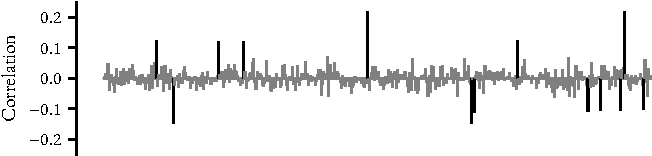
\includegraphics[]{figures/sparse-signal.pdf}
  \caption{%
    A relatively sparse signal. The plot shows standard Pearson correlations between the response vector \(\vec{y}\) and each feature in the \data{madelon} data set~\parencite{guyon2004}. Correlations above 0.1 have been colored in black, the rest in gray.
  }
  \label{fig:sparse-signal}
\end{figure}

We call this hope the \emph{sparsity assumption}. And it can be motivated through the \emph{bet-on-sparsity principle}: assume that the underlying model is sparse and use a sparse method to model it. If the assumption is correct, then our method has a chance of doing well. But if the assumption is incorrect, then our method will not work---but no other method would~\parencite{hastie2009}.

The success of neural networks and other complex models that model high-dimensional data well yet do not enforce sparsity does raise questions as to the validity of this principle. But in our setting, which, loosely speaking, is \emph{explainable} methods for regression, it still bears relevance.

Technically speaking, we are interested in data sets that are made up of a \(n \times p\) matrix of features \(\mat{X}\) and a response vector of length \(n\), \(\vec{y}\):
\[
  \mat{X} = \begin{bmatrix}
    1.5     & 0.3     & \cdots & x_{1,p} \\
    -0.9    & 0.1     & \cdots & x_{2,p} \\
    \vdots  & \vdots  & \ddots & \vdots  \\
    x_{n,1} & x_{n,2} & \cdots & x_{n,p} \\
  \end{bmatrix},\qquad
  \vec{y} = \begin{bmatrix}0.2 \\ -0.9 \\ \vdots \\ y_n\end{bmatrix},
\]
where we have inserted some arbitrary values for the sake of illustration. The data presented in \Cref{tab:types-of-data} corresponds to \(\mat{X}\) here.

In the simplest case, we assume that \(\vec{y}\) is a linear combination of the features in \(\mat{X}\) plus some noise, for instance measurement noise, which we write mathematically as
\[
  \vec{y} = \mat{X}\vec{\beta} + \beta_0 + \vec{\varepsilon},
\]
where \(\vec{\beta}\) is a vector of coefficients and \(\beta_0\) the \emph{intercept}. In this representation of the data, the coefficients \(\vec{\beta}\) are the parameters that we are interested in estimating and represent the effect each feature has on the response vector \(\vec{y}\).

Assuming this model is correct, a natural choice of model to fit this data with is linear regression, which is in fact exactly the model above provided that we, in addition, also assume that the noise \(\vec{\varepsilon}\) is normally distributed\footnote{Tecnically, this not in fact a core assumption of linear regression, but it is necessary for certain aspects of it.} with mean zero and constant variance.

Since in the presence of noise there generally exists no \(\beta\) that will fit the data perfectly, we must accept that the model is only an approximation. The natural follow-up question is then: what \emph{is} a good approximation? To answer this question, we need to define some measure of error. The most common measure, at least as far as linear regression models go, is by far the sum of squared errors between the predicted response vector
\[
  \hat{\vec{y}} = \mat{X}\hat{\vec{\beta}}
\]
and the true response vector \(\vec{y}\), that is
\[
  \lVert \vec{y} - \hat{\vec{y}}\rVert^2_2 = \sum_{i=1}^n (y_i - \hat{y}_i)^2.
\]
The smaller this measure, the better the fit. Which means that we can pose the problem of finding the best model as the following optimization problem:
\begin{problem}
\label{pb:ols}
\begin{aligned}
   & \text{minimize} &  & \frac{1}{2} \lVert \vec{y} - \mat{X}\vec{\beta}\rVert^2_2.
\end{aligned}
\end{problem}
The factor of \(1/2\) is included for convenience, for reasons that will become clear later on.
This choice leads to the ordinary least-squares (OLS) regression model, which, for a simple case of a single feature, we have illustrated in \Cref{fig:ols}. There are many other ways to measure error, which all lead to different models, but in this thesis we will focus on the method of least squares.

The most common linear regression model is ordinary least-squares regression~(OLS), in which we  then the model that minimizes the sum of the squared residuals between the response vector \(\vec{y}\) and the predictions (\(\hat{\vec{y}}\)) made by the model. For the simple case of a single feature, this model is illustrated in \Cref{fig:ols}.

\begin{figure}
  \centering
  \subcaptionbox{%
    The slope of the orange line is \(\beta\). The point where the line intersects the y-axis is the intercept \(\beta_0\).
  }{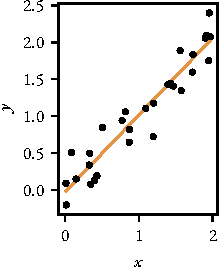
\includegraphics[]{figures/ols-clean.pdf}}\hspace*{1cm}%
  \subcaptionbox{%
    The dotted lines are the residuals and the grey squares are the squared errors.
  }{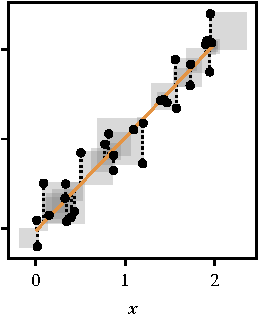
\includegraphics[]{figures/ols-squares.pdf}}
  \caption{%
    Simple ordinary least-squares linear regression for a one-feature problem. }
  \label{fig:ols}
\end{figure}

If have many more observations than features (\(n \gg p\)), then this model might just do. But if we have many more features than observations (\(p \gg n\)), then we have a problem. The problem is that the model will be able to fit the data perfectly, but it will not generalize well to new data. This is because the model will be able to fit the noise in the data, and not the underlying signal. This is called \emph{overfitting}. In fact, the coefficients \(\beta\) will not even be unique in this case.

\begin{figure}
  \centering
  \subcaptionbox{%
    With one fature, the simple ordinarly least-squares regression line fits the data perfectly.
  }{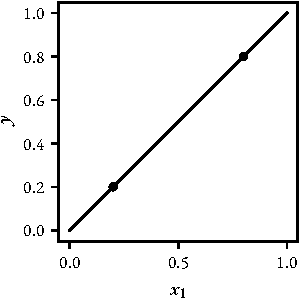
\includegraphics[]{figures/overfit-2d.pdf}}\hfill%
  \subcaptionbox{%
    With two features, multiple fits (planes) will fit the data perfectly.
  }{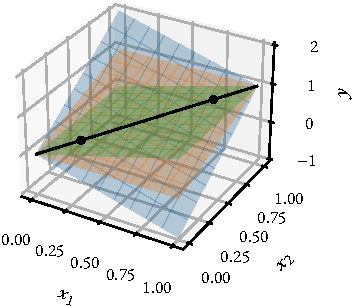
\includegraphics[]{figures/overfit-3d.pdf}}
  \caption{%
    A linear regression problem with two observations
  }
  \label{fig:overfitting}
\end{figure}

The problem illustrated by \Cref{fig:overfitting} is partly one of interpretation. If there are multiple sets of \(\beta\) that will work as well, what do we infer about our parameters?
It is also a case of the curse of dimensionality, in the sense that, as we increase the dimensions of our feature space, our observations start to effectively grow further, and further apart, and occupy less and less of the available space.

In principle, the problem is one of over-parametrization. We have too many parameters for the amount of data that we have. This is, in principle, the same problem that one faces when fitting polynomial regresssion with an increasing number of degress. Eventually the model becomes too flexible and overfits~(\Cref{fig:polyfit}).

\begin{figure}
  \centering
  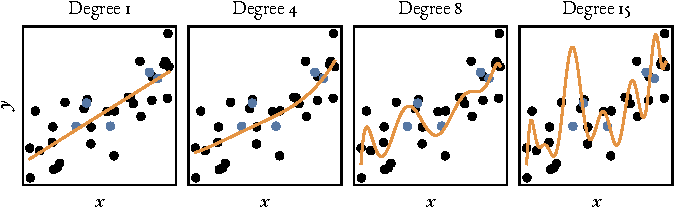
\includegraphics[]{figures/polyfit.pdf}
  \caption{%
    Polynomial regression of a one-feature regression problem.
    The data is generated from the simple linear model \(y_i = 2x_i + \varepsilon\),
    where \(\varepsilon \sim \normal(0, 0.5^2)\).
    The fits to the data become increasingly good as the degree of the polynomial increases, but when new data arrives (the blue points), we see that the model does not generalize well.
  }
  \label{fig:polyfit}
\end{figure}

These problems are the motivation for the use of \emph{regularization} in regression, which we will turn to next.

\section{Regularization}

If the problem is that our model is over-parameterized, which we in the previous section saw is invariably the case when we employ linear regression in the \(p \gg n\) scenario, an intuitive solution might be to restrict or altogheter remove some of the parameters. This is the idea behind \emph{regularization}.

On the surface, this might seem like an awkward idea, since we are in some sense discarding information. But this is exactly what people in the \(n \gg p\) have already done, but at a subjective level. The world is unquestionably high-dimensional and any situation in which we limit the number of features is only an artefact of how we have chosen to measure it. And if we are in the \(n \gg p\) regime, it only means that we have already decided that some features are not important.

Regularization takes another stab at this problem and relies on data, rather than subjective knowledge, in order to choose which features it is that actually matter for the model.

The simplest kind of regularization is called \emph{best-subset selection}, in which we simply set a limit on how many features we allow in our model and fit all possible combinations of models until we find the one that best fits our data. Best subset selection can formally be posed as the following optimzation problem:
% TODO: introduce the minimization objective for OLS somewhere before this
\[
  \begin{aligned}
     & \text{minimize}   &  & \frac{1}{2} \lVert \vec{y} - \mat{X}\vec{\beta}\rVert^2_2, \\
     & \text{subject to} &  & \lVert \vec{\beta} \rVert_0 \leq k,
  \end{aligned}
\]
where \(k\) denotes the number of features that we allow in our model. The \(\lVert \cdot \rVert_0\) norm\footnote{Technically, it's not actually a real norm.} is the number of non-zero elements in a vector.

In other words, if \(k = 2\) and \(p = 3\), for instance, the following models would satisfy our constraints:
\[
  \vec{\beta} = \begin{bmatrix}0 \\ 0 \\ 0\end{bmatrix},\qquad \vec{\beta} = \begin{bmatrix}1 \\ 2 \\ 0\end{bmatrix},\qquad \text{and} \qquad \vec{\beta} = \begin{bmatrix}0 \\ 0 \\ 1\end{bmatrix}.
\]
But the following model would not:
\[
  \vec{\beta} = \begin{bmatrix}1 \\ 2 \\ 3\end{bmatrix}.
\]


There are two problems with this method. The first is that the method involves no shrinkage, which \textcite{stein1956,james1961} in pivotal work asserted was necessary for good performance.

The second is that it is computationally infeasible for large problems. The reason is that the problem is combinatorial and the number of possible models hence grows exponentially with the number of features. Interestingly, \textcite{bertsimas2016} has shown that the problem can actually be written as a mixed-integer optimization problem, which enables the use of modern optimization software. While this is a significant advancement, however, it is still the case that the problem is computationally infeasible for large problems~\parencite{hastie2020}.

% For this thesis, we are in general interested in fitting regularized statistical models to tabular data consisting of a matrix of features (or predictors) \(\mat{X} \in \mathbb{R}^{n \times p}\) and a response vector \(\vec{y} \in \mathbb{R}^n\).
%
% The models that we are interested in fitting are of the form
%
% \begin{align*}
%   \text{minimize} & f(\vec{\beta}; \mat{X}, \vec{y}) = g(\vec{\beta}; \mat{X}, \vec{y}) + h(\vec{\beta})
% \end{align*}
% where \(f(\beta)\)

\subsection{The Lasso}

The perhaps most obvious solution to this problem is to relax the constraint involved in the best-subset selection problem to something that makes the problem easier to solve. And in fact, the closest we can get to the best-subset selection problem without actually solving it is to use the \(\ell_1\) norm in place of the \(\ell_0\) norm. In other words, our problem now becomes
\begin{problem}
\label{pb:lasso}
\begin{aligned}
   & \text{minimize}   &  & \frac{1}{2} \lVert \vec{y} - \mat{X}\vec{\beta}\rVert^2_2, \\
   & \text{subject to} &  & \lVert \vec{\beta} \rVert_1 \leq t,
\end{aligned}
\end{problem}
where \(\lVert \vec{\beta}\rVert_1 = \sum_{j=1}^p |\beta_j|\) and, as a consequence, we have replaced the integer-valued \(k\) with a real-valued (but positive) \(t\). This problem is known as \(\ell_1\)-regularized regression or, more commonly, the \emph{lasso}~\parencite{tibshirani1996}\footnote{The lasso is sometimes written as an acronym (LASSO) for \emph{least absolute shrinkage and selection operator}, but we will stick with the lower-case version here, which the authors themselves use in their recent work.}.

The lasso was introduced to the statistics community by \textcite{tibshirani1996} but actually stems from much earlier research done in the field of signal processing by \textcite{santosa1986}. \textcite{donoho1994,donoho1995} subsequently introduced the concept of the \emph{basis pursuit} problem, which is closely related to the lasso, and developed much of the theoretical framework for the lasso.

We saw previously that the \(\ell_0\) constraint in best-subset selection puts a budget on the number of features allowed in the model. The \(\ell_1\) norm, in contrast, instead puts a budget on the \emph{size} of the coefficients. This leads to both sparsity and shrinkage in the solution. In \Cref{fig:lasso-ball}, we have visualized how this constraint affects the solution of the least-squares objective.

\begin{figure}
  \centering
  \subcaptionbox{A sparse solution, \(\vec{\beta}=[0,-1]^\intercal\).}{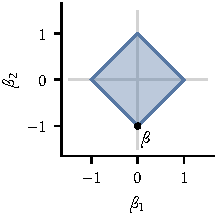
\includegraphics[]{figures/lasso-ball-sparse.pdf}}\hfill%
  \subcaptionbox{A dense solution, \(\vec{\beta}=[0.5,0.5]^\intercal\).}{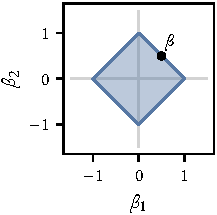
\includegraphics[]{figures/lasso-ball-dense.pdf}}\hfill%
  \subcaptionbox{A solution in which the constraint is inactive, \(\vec{\beta} = [0.4,0.3]^\intercal\). \(t\) is too small to have any effect on the solution.}{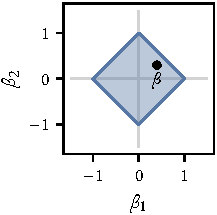
\includegraphics[]{figures/lasso-ball-inactive.pdf}}

  \caption{%
    The \(\ell_1\) norm ball in \(\mathbb{R}^2\) with some possible solutions indicated by \(\vec{\beta}\). The \(\ell_0\) ball (for best-subset selection) and \(k = 1\) would be lines of infinite length. along both of the axes.
  }
  \label{fig:lasso-ball}
\end{figure}

There is now an extensive body of work on the lasso and it has spawned many different variants, such as the fused lasso~\parencite{tibshirani2005}, group lasso~\parencite{yuan2005}, adaptive lasso~\parencite{zou2006}, graphical lasso~\parencite{friedman2008}, and square-root lasso~\parencite{belloni2011}. In this thesis, however, we will focus on the standard lasso.

Note, also, that the lasso is also not limited to regularized \emph{linear} regression but can also be used for the entire family of generalized linear models, such as logistic, Poisson, multinomial, and multivariate regression, as well as survival models such as Cox regression. The use of the \(\ell_1\)-norm penalty has also found its way into many other areas of statistics, signal processing, and machine learning, such as matrix factorization, clustering, and deep learning.

An interesting property of the lasso is that it is possible (and computationally feasible) to exactly solve the lasso problem for all possible values of \(t \in [0, \infty)\). This is commonly referred to as the \emph{lasso path}~(\Cref{fig:lasso-path}). It begins at \(t=0\), for which the constraint region is a point, which forces all of the coefficients to be exactly zero. As \(t\) increases, the constraint region grows, allowing the coefficients to enter the model. The reason for why it is possible to solve for the full path is that the solution vector \(\beta\), as a function of \(t\), is linear and continuous between the values of \(t\) for which features enter or leave the model.

\begin{figure}
  \centering
  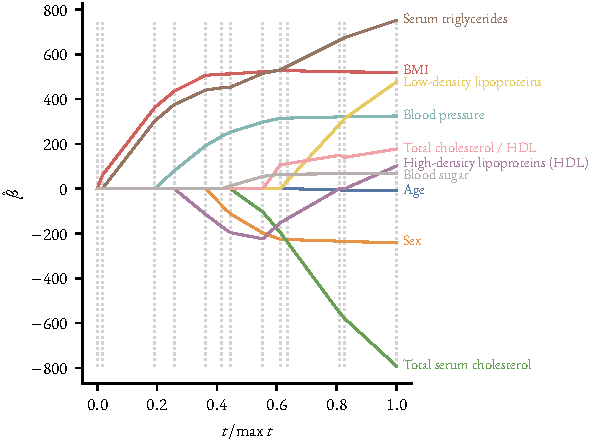
\includegraphics[]{figures/lasso-path.pdf}
  \caption{%
    The lasso path for the \data{diabetes} data set~\parencite{efron2004}, which consists of \(n=442\) observations and \(p=10\) features. The path shows the coefficients as a function of the parameter \(t\), which controls the size of the constraint region. The path is piecewise linear with kinks ocurring only when features enter or exit the model.}
  \label{fig:lasso-path}
\end{figure}

A problem with the lasso, however, is that it does not deal with the case of correlated features as intuitiion (at least that of the author) would suggest. If two features are correlated highly ``enough'', the lasso will select one of them and set the other to zero. This is not a problem for the predicted response \(\hat{\vec{y}}\), but it means that the estimated coefficients \(\hat{\vec{\beta}}\) no longer provide a trustworthy estimate of variable (feature) importance. This effect is the result of the behavior of the \(\ell_1\) norm, which penalizes the size of the coefficients. If two features provide the same, or nearly the same, information about the response, then the optimization problem can attain a lower value by setting one of the coefficients to zero.

This is a problem that the \emph{elastic net}---the topic of the next section---is designed to overcome.

\subsection{The Elastic Net}

The elastic net is a combination of the lasso and ridge regression\footnote{Ridge regression is also known as Tikhonov regression.}, which can be written as the following optimization problem:
\[
  \begin{aligned}
     & \text{minimize}   &  & \frac{1}{2} \lVert \vec{y} - \mat{X}\vec{\beta}\rVert^2_2,                             \\
     & \text{subject to} &  & \alpha \lVert \vec{\beta} \rVert_1 + (1-\alpha) \lVert \vec{\beta}\rVert_2^2 \leq t_1, \\
  \end{aligned}
\]
The difference compared to the lasso is that we transformed our constraint into a linear combination of the \(\ell_1\) and \(\ell_2\) norms. Setting \(\alpha = 1\), the problem would once again become the lasso. With \(\alpha = 0\), we would instead have ridge regression. Any value \(\alpha \in (0, 1)\) yields a combination of the two~(\Cref{fig:elasticnet-balls}).

\begin{figure}[htpb]
  \centering
  \subcaptionbox{%
    When \(\alpha = 1\), the constraint is
    the lasso (\(\ell_1\)-norm) ball. And in this case the solution is sparse.
  }{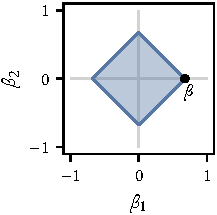
\includegraphics{figures/elasticnet-balls-lasso}}\hfill%
  \subcaptionbox{%
    When \(\alpha = 0\), the constraint is the ridge (\(\ell_2\)-norm) ball. Here, the solution is not sparse.
  }{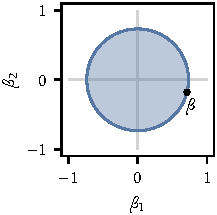
\includegraphics{figures/elasticnet-balls-ridge}}\hfill%
  \subcaptionbox{%
    When \(\alpha \in (0, 1)\), the constraint region is a combination of the \(\ell_1\) and \(\ell_2\) balls. In this case we have \(\alpha=1/2\). Once again, the solution is sparse.
  }{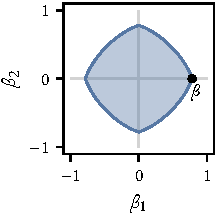
\includegraphics{figures/elasticnet-balls-elasticnet}}
  \caption{%
    The constraint regions for the elastic net for different values of \(\alpha\)
  }
  \label{fig:elasticnet-balls}
\end{figure}

The elastic net was first proposed by \textcite{zou2005}. In addition to dealing with the problems encountered in using the lasso for highly correlated features, the elastic net also yields improved predictive performance in many situations. The latter fact is perhaps not so surprising given that it is a combination of methods that essentially assume different structure in the data. The lasso undoubtably works best when the true signal is sparse, while ridge regression handles the situation where there are weak signals better. It is then quite natural that there should for many data sets exist a \(\alpha\) that is smaller than one but larger than zero that yields the best performance.

\subsection{SLOPE}

Another way of dealing with the problem of correlated features is to use \emph{Sorted L-One Penalized Estimation} (SLOPE)~\parencite{bogdan2013,zeng2014,bogdan2015}. SLOPE is a generalization of both the lasso and \emph{the octagonal shrinkage and clustering algorithm for regression} (OSCAR)~\parencite{bondell2008}. It is represented by the following optimization objective:
\[
  \begin{aligned}
     & \text{minimize}   &  & \frac{1}{2} \lVert \vec{y} - \mat{X}\vec{\beta}\rVert^2_2, \\
     & \text{subject to} &  & \sum_{j=1}^p w_i |\beta|_{(i)} \leq t,
  \end{aligned}
\]
where \(\vec{w}\) is a non-increasing and non-negative sequence of penalization weights and
where we define the subscript operator \((i)\) such that
\[
  |\beta|_{(1)} \geq |\beta|_{(2)} \geq \cdots \geq |\beta|_{(p)}.
\]
The left-hand side of the constraint in SLOPE is, perhaps somewhat surprisingly, actually a norm: the \emph{sorted \(\ell_1\) norm}.

The perhaps most salient feature of SLOPE is that it clusters coefficients~\parencite{figueiredo2014,schneider2022}. Please refer to \Cref{fig:slope-balls} for an example of this. This makes it perfectly fit to handle the case when features are highly correlated, which he highlighted as an issue of the lasso before. If the lasso set one of the coefficients to zero, SLOPE will instead set them to exactly the same value (in absolue terms). This is a property that is not shared by the elastic net, which handles correlation (although not quite as delicately), but does not cluster coefficients.

But as we mentioned previously, SLOPE is actually a generalization of lasso and thus contains it as a special case~(\Cref{fig:slope-balls-lasso}), which is attained by setting all of the elements of the penalization weight vector \(\vec{w}\) to the same value. On the opposite end, setting only the first element to a non-zero value and the remaining ones to zero yields the infinity norm~(\Cref{fig:slope-balls-inf}). The latter is not of particular interest in practice.

\begin{figure}[htpb]
  \centering
  \subcaptionbox{%
  When \(\vec{w} = [1, 1]^\intercal\), the constraint region is the lasso ball, \(\lVert \vec{\beta}\rVert_1\).\label{fig:slope-balls-lasso}
  }{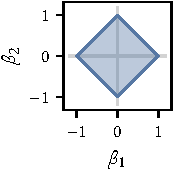
\includegraphics{figures/slope-ball-0.pdf}}\hfill%
  \subcaptionbox{%
  Here we have \(\vec{w} = [1, 3/4]^\intercal\), but no clustering occurs.
  }{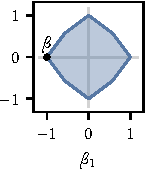
\includegraphics{figures/slope-ball-1.pdf}}\hfill%
  \subcaptionbox{%
  With \(\vec{w} = [1, 1/4]^\intercal\), the solution is now clustered.
  }{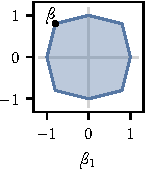
\includegraphics{figures/slope-ball-2.pdf}}\hfill%
  \subcaptionbox{%
  When \(\vec{w} = [1, 0]^\intercal\), the constraint is the infinity norm, \(\lVert \vec{\beta}\rVert_\infty\).\label{fig:slope-balls-inf}
  }{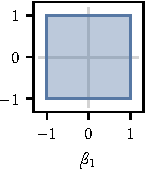
\includegraphics{figures/slope-ball-3.pdf}}
  \caption{%
    SLOPE balls (the sorted \(\ell_1\) norm) for various choices of the penalization weight vector \(\vec{w}\). It is the kinks at the boundaries, ocurring when \(|\beta_1| =|\beta_2|\), that induce clustering. The larger the difference between adjacent values in \(\vec{w}\), the stronger the clustering effect becomes.
  }
  \label{fig:slope-balls}
\end{figure}

SLOPE also has other appealing properties, such as the ability to (under certain assumptions on the design) control of false discovery rate\footnote{In terms of the number of coefficients correctly identified as non-zero over the number of total discoveries (selected features).}~\parencite{bogdan2015} and recover of sparsity and ordering patterns in the solution~\parencite{bogdan2022}. Another key feature is that the problem is also convex, which has implications that we will delve into later. And it puts SLOPE apart from other more complicated models such as minimax concave penalty (MCP)~\parencite{zhang2010} and smoothly clipped absolute deviation (SCAD)~\parencite{fan2001}.

We have so far only discussed the models that we are interested in fitting, but have said nothing about \emph{how} we fit them. We will turn to this issue in the next section.

% \section{Solving the Problems}
\section{Optimization}\label{sec:optimization}

In the previous section we introduced the bulk of the statistical models this thesis will revolve around. They certainly have many interesting theoretical properties, which we have only touched upon briefly, but it is actually not the statistical theory of these problems that we will concern ourselves with in this thesis. Instead, we will be interested in the \emph{numerical} aspects of these problems. That is: how do we actually solve them? And, moreover, how do we do this as efficiently as possible?

We have already introduced many optimization problems and have more or less assumed that we can solve them. This assumption is by no means wrong: methods for fitting the lasso, elastic net, and SLOPE are readily available for free in many programming languages and can be installed via a few lines of code. For instance, to fit the full lasso path to the \data{diabetes} data that we ecountered previously~(see \Cref{fig:lasso-path} for the result), we only need to call the following \lang{R} code.

\begin{lstlisting}[language=R]
library(lars)

data(diabetes)
fit <- lars(diabetes$x, diabetes$y, type = "lasso")
\end{lstlisting}

Behind the scenes, however, the method invoked through this command actually involve a complicated optimization algorithm into which considerable effort has been put in order to ensure that what you get in \texttt{fit} is reliable---and that you get it \emph{fast}.

\subsection{Direct Methods}

The first optimization problem that we encountered in this text was ordinary least-squares regression, which we formally defined in \Cref{pb:ols}. Naively speaking, the solution to this problem is actually relatively straightforward. Letting
\[
  f(\vec{\beta}) = \frac{1}{2}\lVert \vec{y} - \mat{X}\vec{\beta}\rVert_2^2
\]
be the objective function that we want to minimize, we simply set the gradient of it to zero:
\[
  \begin{aligned}
    \nabla f(\vec{\beta})                & = \mat{X}^\intercal (\mat{X}\vec{\beta} - \vec{y}) = \zeros \implies \\
    \mat{X}^\intercal \mat{X}\vec{\beta} & = \mat{X}^\intercal \vec{y}.
  \end{aligned}
\]
This system\footnote{We have ignored the intercept \(\beta_0\) here for simplicity, but it could be incorporated easily by prepending a vector of ones to \(\mat{X}\).} is called the \emph{normal equations}. Solving the system in \(\beta\) yields the ordinary least squares estimate, which, for a one-dimensional problem is equivalent to locating the ``bottom'' of the function \(f(\beta)\) in \Cref{fig:1dconvexity-convex}. It might be tempting to want to simply invert \(\mat{X}^\intercal\mat{X}\) here and premultiply by both sides to yield an explicit solution of the form
\[
  \vec{\beta} = (\mat{X}^\intercal\mat{X})^{-1}\mat{X}^\intercal\vec{y}
\]
but this is typically a bad idea since the inverse need not exist or be numerically stable. A better option is to use a method such as the QR decomposition and solve the resulting system through forward or backwards elimination, which is both more stable and more efficient, and all modern software use some variation of this approach.

Regardless, however, OLS can be solved directly and with accuracy at machine precision. This property is shared by ridge regression in which we can attain a solution simply by adding a diagonal matrix\footnote{This procedure referes to the \emph{unconstrained} form of ridge regression, which have not yet---but will soon---introduce.} to \(\mat{X}^\intercal\mat{X}\) and solving as before. The key reason for why this is the case is that OLS is a differentiable and quadratic problem, which means that it is \emph{convex} and hence has a global solution~(\Cref{fig:1dconvexity-convex}), unlike, for instance, the problem in \Cref{fig:1dconvexity-nonconvex}, which is non-convex (actually a third-degree polynomial) and hence has a local minimum.

\begin{figure}
  \centering
  \subcaptionbox{A convex and smooth function. The minimum ocurs when \(\nabla f(\beta) = 0\).\label{fig:1dconvexity-convex}}{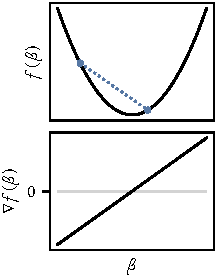
\includegraphics[]{figures/1d-convexity-convex.pdf}}\hfill%
  \subcaptionbox{A non-convex but smooth function. The derivative offers no information about the global minimum (which is \(-\infty\)).\label{fig:1dconvexity-nonconvex}}{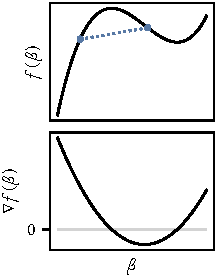
\includegraphics[]{figures/1d-convexity-nonconvex.pdf}}\hfill%
  \subcaptionbox{A convex but non-smooth function. There is a global minimum, but the derivative does not exist at this point.\label{fig:1d-convexity-nonsmooth}}{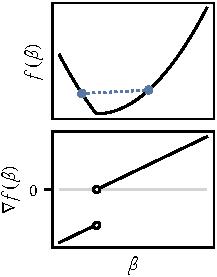
\includegraphics[]{figures/1d-convexity-nonsmooth.pdf}}
  \caption{%
    Three different kinds of functions. We show the objective value \(f(\beta)\) and the gradient \(\nabla f(\beta)\) for each. In each case, our objective is to find the minimum of the function. Only the first and last are convex (the complete line segment between two points on the function lies above the function) and have a global minimum.
  }
  \label{fig:1d-convexity}
\end{figure}

All the problems that we have covered so far: ordinary least-squares regression, the lasso, the elastic net, and SLOPE are all convex problems, which is the class of problems this thesis focuses on. Being convex, however, does not necessarily mean that the problem is easy to solve. The lasso~(\Cref{pb:lasso}), for instance, is a convex problem, but the involvement of the inequality constraint means that we cannot solve it directly, at least not for any given \(t\).

Somewhat remarkably, however, there actually exist methods that \emph{can} solve the full lasso path directly, which means they can also indirectly solve the lasso for a single \(t\). This class of methods are called \emph{homotopy algorithms} since they solve the problem for all values they are parameterized by (in this case \(t\)). The first homotopy method for the lasso was introduced by \textcite{osborne2000a} but it is the LARS algorithm~\parencite{efron2004}, that we already saw in action at the beginning of the section, which popularized the method.

In essence, homotopy methods for lasso are based on the idea that the lasso can be solved directly if we know the support of the solution (the identity of the non-zero coefficients). Based on this idea, we start with the empty support at \(t=0\). From this point, it is possible to say which feature(s) will become active first and then solve the problem (directly) for this support set. We can then proceed to the next support set, rinse, and repeat. We give a rough, but slightly more formalized, description of the method in \Cref{alg:homotopy}.

\begin{algorithm}
  \caption{A rough outline of the homotopy method for the lasso path. The steps in lines 3 and 4 represent the critical aspect of the algorithm, and are omitted here for brevity, but they are not particularly demanding computationally. The costs come from the number of iterations that are needed to solve the entire path.}
  \label{alg:homotopy}
  \KwIn{$\vec{\beta}^{(0)} \gets \zeros$, $t \gets 0$, $\mathcal{A} \gets \emptyset$, $i \gets 0$}
  \Repeat{$|\mathcal{A}| = p$}{
  $i \gets i + 1$\;
  $t \gets$ next value for which the support changes\;
  $\mathcal{A} \gets$ support at $t$\;
  $\vec{\beta}^{(i)}_{\mathcal{A}} \gets \arg\min_{\vec{\beta} \in \mathbb{R}^{|\mathcal{A}|}} f(\vec{\beta})$\;
  $\vec{\beta}^{(i)}_{\mathcal{A}^C} \gets \zeros$\;
  }
\end{algorithm}

At the time that these methods were introduced, they offered a remarkable boost in efficiency compared to the original algorithm used by \textcite{tibshirani1996}, which consisted of an iterative method based on an algorithm by \textcite{lawson1995}. This method scaled badly with \(p\) and was altogether inapplicable when \(p > n\).

It is a well-known fact that the elastic net can be recast as a lasso problem, which means that the homotopy methods for the lasso can be used for the elastic net as well. There also exists homotopy methods for SLOPE~\parencite{nomura2020,dupuis2023}, since SLOPE shares the piecewise-linear property of the lasso path (although the SLOPE path is typically more complicated, with even more kinks).

Even if these homotopy methods provided a much-wanted upgrade compared to the original method for the high-dimensional regime, it is nevertheless this domain that they ultimately struggle to deal with. The root of this problem is that there are at least \(\min(n,p)\) changes in support along the full lasso path---and in the worst case as many as \((3^p + 1)/2\) such changes~\parencite{mairal2012}. The algorithm has to solve an equivalent number of OLS problems, albeit at a complexity much reduced from that of solving the full problem, which, in the end, means that the method has found itself outperformed by iterative optimization methods~\parencite{friedman2010}, which we will introduce in the next section, starting with \emph{proximal gradient descent}.

% TODO: if time permits, consider saying something about methods for constrained optimization.

\subsection{Proximal Gradient Descent}

but it is also non-smooth, which means that the gradient does not exist everywhere. The problem in \Cref{fig:1d-convexity-nonsmooth} is actually corresponds to a one-dimensional lasso problem where the optimum is achieved at a point where the derivative does not exist.


\section{Screening Rules}\label{sec:screening-rules}

\section{Normalization}

\section{Summary of the Papers}

\subsection{Paper \I}

In this paper, we address the challenge of extracting relevant features from data sets where the number of observations, n, is significantly smaller than the number of predictors, p. We focus on the Sorted L-One Penalized Estimation (SLOPE)—a generalization of the lasso—as a promising method in this context. However, current numerical procedures for SLOPE lack the efficiency that lasso tools possess, especially when estimating a complete regularization path. A key component of lasso's efficiency is predictor screening rules, which allow predictors to be discarded before model estimation. This paper is the first to establish such a rule for SLOPE. We develop a SLOPE screening rule by examining its subdifferential and demonstrate that this rule is a generalization of the strong rule for the lasso. Although our rule is heuristic and may occasionally discard predictors erroneously, we show that such instances are rare and can be easily safeguarded against by a simple check of the optimality conditions. Our numerical experiments reveal that the rule performs well in practice, leading to significant improvements for data in the \(p \gg n\) domain, and incurs no additional computational overhead when \(n > p\). This paper, therefore, presents a significant advancement in the efficiency of SLOPE, particularly in high-dimensional settings.

\subsection{Paper \II}

In this paper, we focus on the lasso, a widely used method for inducing shrinkage and sparsity in the solution vector of regression problems, especially when the number of predictors outweighs the number of observations. Solving the lasso in such high-dimensional settings can be computationally challenging. However, this challenge can be mitigated through the use of screening rules that discard predictors before fitting the model, resulting in a reduced problem. We introduce a new screening strategy, termed look-ahead screening. This method employs safe screening rules to identify a range of penalty values for which a specific predictor cannot enter the model, thereby screening predictors along the remaining path. Our experiments demonstrate that these look-ahead screening rules outperform the active warm-start version of the Gap Safe rules, marking a significant advancement in the efficiency of solving high-dimensional lasso problems.

\subsection{Paper \III}

In this paper, we address the challenge of predictor screening rules in l1-regularized regression problems, such as the lasso. These rules, which eliminate predictors from the design matrix before fitting a model, have significantly improved the speed of solving such problems. However, current state-of-the-art screening rules struggle with highly-correlated predictors, often becoming overly conservative. To tackle this issue, we introduce a new screening rule: the Hessian Screening Rule. This rule leverages second-order information from the model to provide more accurate screening and higher-quality warm starts. Our proposed rule outperforms all other alternatives we studied on datasets with high correlation for both l1-regularized least-squares (the lasso) and logistic regression. It also delivers the best performance overall on the real datasets we examined. This paper, therefore, presents a significant advancement in dealing with highly-correlated predictors in l1-regularized regression problems.

\subsection{Paper \IV}

In this paper, we tackle the challenges posed by the rapid development of machine learning research, particularly in the area of numerical validation. Researchers often face a multitude of methods to compare, lack of transparency and consensus on best practices, and the tedious task of re-implementing work. This often results in partial validation, which can lead to incorrect conclusions and hinder research progress. To address these issues, we introduce Benchopt, a collaborative framework designed to automate, reproduce, and publish optimization benchmarks in machine learning across different programming languages and hardware architectures. Benchopt simplifies the benchmarking process by providing a ready-to-use tool for running, sharing, and extending experiments. We demonstrate its wide applicability through benchmarks on three standard learning tasks: $\ell_2$-regularized logistic regression, Lasso, and ResNet18 training for image classification. These benchmarks reveal key practical findings that provide a more nuanced view of the state-of-the-art for these problems, emphasizing that the details matter in practical evaluation. We believe that Benchopt will encourage collaborative work in the community and improve the reproducibility of research findings.

\subsection{Paper \V}

In this paper we delve into the Sorted L-One Penalized Estimation (SLOPE), an extension of the renowned lasso regression method. Despite the promising statistical properties of SLOPE, its adoption has been limited due to the inefficiency of existing algorithms in high-dimensional contexts. To overcome this challenge, we introduce a novel, faster algorithm that solves the SLOPE optimization problem.

Our algorithm merges the techniques of proximal gradient descent and proximal coordinate descent, significantly enhancing the efficiency of the SLOPE method. We also shed new light on the directional derivative of the SLOPE penalty and its associated SLOPE thresholding operator, and provide assurances of convergence for our proposed solver. Through comprehensive benchmarks on both simulated and real data, we demonstrate that our method outperforms a host of competing algorithms. This paper is a significant contribution as it broadens the applicability of the SLOPE method in high-dimensional settings, potentially paving the way for its wider use in the field.

\subsection{Paper \VI}

In this paper, we explore the sensitivity of regularized methods, such as the lasso and ridge regression, to the scales of the features in the data. It's standard practice to normalize features to ensure they share the same scale. While standardization is common for continuous data, binary data, particularly when high-dimensional and sparse, is often not scaled at all. We demonstrate that this choice can significantly impact the estimated model when the binary features are imbalanced, and that these effects also depend on the type of regularization used. Specifically, we show that the size of a feature's corresponding coefficient in the lasso is directly related to its class imbalance, and this effect depends on the normalization used. We propose potential solutions to this issue and discuss the case when data is mixed, containing both continuous and binary features. This paper, therefore, provides valuable insights into the impact of feature scaling on regularized methods and offers practical solutions for handling mixed data.
